%%%%%%%%%%%%%%%%%%%%%%%%%%%%%%%%%%%%%%%%%
% Beamer Presentation
% LaTeX Template
% Version 2.0 (March 8, 2022)
%
% This template originates from:
% https://www.LaTeXTemplates.com
%
% Author:
% Vel (vel@latextemplates.com)
%
% License:
% CC BY-NC-SA 4.0 (https://creativecommons.org/licenses/by-nc-sa/4.0/)
%
%%%%%%%%%%%%%%%%%%%%%%%%%%%%%%%%%%%%%%%%%

%----------------------------------------------------------------------------------------
%	PACKAGES AND OTHER DOCUMENT CONFIGURATIONS
%----------------------------------------------------------------------------------------

\documentclass[
	11pt, % Set the default font size, options include: 8pt, 9pt, 10pt, 11pt, 12pt, 14pt, 17pt, 20pt
	%t, % Uncomment to vertically align all slide content to the top of the slide, rather than the default centered
	%aspectratio=169, % Uncomment to set the aspect ratio to a 16:9 ratio which matches the aspect ratio of 1080p and 4K screens and projectors
]{beamer}

\graphicspath{{Images/}{./}} % Specifies where to look for included images (trailing slash required)

\usepackage{booktabs} % Allows the use of \toprule, \midrule and \bottomrule for better rules in tables

%----------------------------------------------------------------------------------------
%	SELECT LAYOUT THEME
%----------------------------------------------------------------------------------------

% Beamer comes with a number of default layout themes which change the colors and layouts of slides. Below is a list of all themes available, uncomment each in turn to see what they look like.

%\usetheme{default}
%\usetheme{AnnArbor}
%\usetheme{Antibes}
%\usetheme{Bergen}
%\usetheme{Berkeley}
%\usetheme{Berlin}
%\usetheme{Boadilla}
%\usetheme{CambridgeUS}
%\usetheme{Copenhagen}
%\usetheme{Darmstadt}
%\usetheme{Dresden}
%\usetheme{Frankfurt}
%\usetheme{Goettingen}
%\usetheme{Hannover}
%\usetheme{Ilmenau}
%\usetheme{JuanLesPins}
%\usetheme{Luebeck}
\usetheme{Madrid}
%\usetheme{Malmoe}
%\usetheme{Marburg}
%\usetheme{Montpellier}
%\usetheme{PaloAlto}
%\usetheme{Pittsburgh}
%\usetheme{Rochester}
%\usetheme{Singapore}
%\usetheme{Szeged}
%\usetheme{Warsaw}

%----------------------------------------------------------------------------------------
%	SELECT COLOR THEME
%----------------------------------------------------------------------------------------

% Beamer comes with a number of color themes that can be applied to any layout theme to change its colors. Uncomment each of these in turn to see how they change the colors of your selected layout theme.

%\usecolortheme{albatross}
%\usecolortheme{beaver}
%\usecolortheme{beetle}
%\usecolortheme{crane}
%\usecolortheme{dolphin}
%\usecolortheme{dove}
%\usecolortheme{fly}
%\usecolortheme{lily}
%\usecolortheme{monarca}
%\usecolortheme{seagull}
%\usecolortheme{seahorse}
%\usecolortheme{spruce}
%\usecolortheme{whale}
%\usecolortheme{wolverine}

%----------------------------------------------------------------------------------------
%	SELECT FONT THEME & FONTS
%----------------------------------------------------------------------------------------

% Beamer comes with several font themes to easily change the fonts used in various parts of the presentation. Review the comments beside each one to decide if you would like to use it. Note that additional options can be specified for several of these font themes, consult the beamer documentation for more information.

\usefonttheme{default} % Typeset using the default sans serif font
%\usefonttheme{serif} % Typeset using the default serif font (make sure a sans font isn't being set as the default font if you use this option!)
%\usefonttheme{structurebold} % Typeset important structure text (titles, headlines, footlines, sidebar, etc) in bold
%\usefonttheme{structureitalicserif} % Typeset important structure text (titles, headlines, footlines, sidebar, etc) in italic serif
%\usefonttheme{structuresmallcapsserif} % Typeset important structure text (titles, headlines, footlines, sidebar, etc) in small caps serif

%------------------------------------------------

%\usepackage{mathptmx} % Use the Times font for serif text
\usepackage{palatino} % Use the Palatino font for serif text
%\usepackage{helvet} % Use the Helvetica font for sans serif text
\usepackage[default]{opensans} % Use the Open Sans font for sans serif text
%\usepackage[default]{FiraSans} % Use the Fira Sans font for sans serif text
%\usepackage[default]{lato} % Use the Lato font for sans serif text

%----------------------------------------------------------------------------------------
%	SELECT INNER THEME
%----------------------------------------------------------------------------------------

% Inner themes change the styling of internal slide elements, for example: bullet points, blocks, bibliography entries, title pages, theorems, etc. Uncomment each theme in turn to see what changes it makes to your presentation.

%\useinnertheme{default}
\useinnertheme{circles}
%\useinnertheme{rectangles}
%\useinnertheme{rounded}
%\useinnertheme{inmargin}

%----------------------------------------------------------------------------------------
%	SELECT OUTER THEME
%----------------------------------------------------------------------------------------

% Outer themes change the overall layout of slides, such as: header and footer lines, sidebars and slide titles. Uncomment each theme in turn to see what changes it makes to your presentation.

%\useoutertheme{default}
%\useoutertheme{infolines}
%\useoutertheme{miniframes}
%\useoutertheme{smoothbars}
%\useoutertheme{sidebar}
%\useoutertheme{split}
%\useoutertheme{shadow}
%\useoutertheme{tree}
%\useoutertheme{smoothtree}

%\setbeamertemplate{footline} % Uncomment this line to remove the footer line in all slides
%\setbeamertemplate{footline}[page number] % Uncomment this line to replace the footer line in all slides with a simple slide count

%\setbeamertemplate{navigation symbols}{} % Uncomment this line to remove the navigation symbols from the bottom of all slides

%----------------------------------------------------------------------------------------
%	PRESENTATION INFORMATION
%----------------------------------------------------------------------------------------

\title[Computer \& Programming, MATLAB]{ENGR151 Recitation Class 6} % The short title in the optional parameter appears at the bottom of every slide, the full title in the main parameter is only on the title page

\subtitle{week 8} % Presentation subtitle, remove this command if a subtitle isn't required

\author[Wu JiaXi]{Wu JiaXi} % Presenter name(s), the optional parameter can contain a shortened version to appear on the bottom of every slide, while the main parameter will appear on the title slide

\institute[UM-SJTU joint institute]{UM-SJTU joint institute \\ \smallskip \textit{nina$\_$nhk@sjtu.edu.cn}} % Your institution, the optional parameter can be used for the institution shorthand and will appear on the bottom of every slide after author names, while the required parameter is used on the title slide and can include your email address or additional information on separate lines

\date[\today]{Computer $\&$ Programming, MatLab-scripting \\ \today} % Presentation date or conference/meeting name, the optional parameter can contain a shortened version to appear on the bottom of every slide, while the required parameter value is output to the title slide

%----------------------------------------------------------------------------------------

\begin{document}

%----------------------------------------------------------------------------------------
%	TITLE SLIDE
%----------------------------------------------------------------------------------------

\begin{frame}
	\titlepage % Output the title slide, automatically created using the text entered in the PRESENTATION INFORMATION block above
\end{frame}

%----------------------------------------------------------------------------------------
%	TABLE OF CONTENTS SLIDE
%----------------------------------------------------------------------------------------

% The table of contents outputs the sections and subsections that appear in your presentation, specified with the standard \section and \subsection commands. You may either display all sections and subsections on one slide with \tableofcontents, or display each section at a time on subsequent slides with \tableofcontents[pausesections]. The latter is useful if you want to step through each section and mention what you will discuss.

\begin{frame}
	\frametitle{Presentation Overview} % Slide title, remove this command for no title
	
	\tableofcontents % Output the table of contents (all sections on one slide)
	%\tableofcontents[pausesections] % Output the table of contents (break sections up across separate slides)
\end{frame}


\begin{frame}
	\frametitle{Recording} % Slide title, remove this command for no title
	
	Here is the link for the recording of this RC: \href{https://sjtu.feishu.cn/minutes/obcnw1h35g9wd599qt28pdq7?from=from_copylink}{Click Here}
\end{frame}
----
----------------------------------------------------------------------------------------
	PRESENTATION BODY SLIDES
----------------------------------------------------------------------------------------

\section{Playbook Review} % Sections are added in order to organize your presentation into discrete blocks, all sections and subsections are automatically output to the table of contents as an overview of the talk but NOT output in the presentation as separate slides

%------------------------------------------------
\begin{frame}
	\textbf{Disclaimer:}\\
    The answers provided here are not guranteed to be correct. Please
    use them as a references only and verify with reliable source.

    \smallskip

    \textbf{Note:}\\
     only go through some questions that we think they are necessary.
	
\end{frame}

%------------------------------------------------
\subsection{C7}


\begin{frame}{C7 review 7.1.1}
    \textbf{1. What is the first index in an array?} \\
    In C, the first index of an array is always 0. \\
    \textbf{2. Can we write \texttt{int a[] = \{1, 2, 3, 4\}}? Why?} \\
    Yes, this is valid because C allows the compiler to determine the array size based on the number of elements in the initializer. \\
    \textbf{3. Why no braces are used in lines 4-5 of the for loop?} \\
    If a loop body consists of only one statement, braces are optional. \\
\end{frame}


\begin{frame}{C7 review 7.1.2}
    \textbf{1. Why is \texttt{arr[]} used instead of \texttt{arr[5]}?} \\
    \texttt{arr[]} is used because the array size is passed as a separate parameter. It doesn't need to be specified in the function signature. \\
    \textbf{2. What is \texttt{const} and why is it used?} \\
    \texttt{const} makes the \texttt{size} parameter read-only within the function to prevent accidental modification. \\
    \textbf{3. What is \texttt{size\_t} and why is it used?} \\
    \texttt{size\_t} is an unsigned integer type used for array sizes and indexing, ensuring that the size can't be negative. \\
\end{frame}

% 7.1.4

\begin{frame}{C7 review 7.1.4}
    \textbf{1. Why is \texttt{srand(time(NULL))} used?} \\
    \texttt{srand(time(NULL))} seeds the random number generator with the current time to ensure a different sequence of random numbers each time the program runs. \\
    \textbf{2. What is \texttt{time.h}?} \\
    \texttt{time.h} is a library providing time and date functions in C. \\
    \textbf{3. How many times does the random seed need to be initialized?} \\
    The random seed should be initialized once at the start of the program. \\
    \textbf{4. Run the program and explain why the result is meaningful.} \\
    The result is meaningful because it simulates the distribution of dice rolls, showing how often each face of the die appears in a series of rolls. \\
\end{frame}

% 7.1.6

\begin{frame}{C7 review 7.1.6}
    \textbf{1. Why should multidimensional arrays be avoided?} \\
    Multidimensional arrays can be more difficult to manage and less memory-efficient. \\
    \textbf{2. Rewrite the code to use a 1-dimensional array.} \\
    \texttt{int table[1000];} \\
    \textbf{3. Increase the number of rolls by adding 0's. What happens?} \\
    Adding 0's could make the simulation behave differently depending on how the array is handled. It may result in invalid memory accesses.
\end{frame}

% 7.2.1

\begin{frame}{C7 review  7.2.1}
    \textbf{1. What are pointers?} \\
    A pointer is a variable that stores the memory address of another variable. \\
    \textbf{2. Are \texttt{int* a} and \texttt{int *a} the same?} \\
    Yes, both notations mean the same: \texttt{a} is a pointer to an integer. \\
    \textbf{3. Meaning of \texttt{*} in \texttt{*a = 5} and \texttt{int* a}?} \\
    In \texttt{*a = 5}, \texttt{*a} dereferences the pointer to assign a value. In \texttt{int* a}, \texttt{*} indicates that \texttt{a} is a pointer. \\
    \textbf{4. Double pointer and triple pointer illustration:} \\
    \texttt{int **p;} points to a pointer, and \texttt{int ***p;} points to a double pointer. \\
\end{frame}

% 7.2.5

\begin{frame}{C7 review 7.2.5 }
    \textbf{1. What is \texttt{float **xp2} and why is it used?} \\
    \texttt{xp2} is a pointer to a pointer. It holds the address of a pointer variable. \\
    \textbf{2. Where is \texttt{xp1} pointing?} \\
    \texttt{xp1} is pointing to the variable \texttt{x}. \\
    \textbf{3. Why is the compiler issuing a warning?} \\
    The warning may be due to using the wrong format specifier for pointer types in \texttt{printf}. \\
\end{frame}

% 7.2.6

\begin{frame}{C7 review 7.2.6}
    \textbf{1. Why should the size of the element be specified in \texttt{malloc()}?} \\
    This ensures that the correct amount of memory is allocated for each element. \\
    \textbf{2. What is a memory leak?} \\
    A memory leak occurs when dynamically allocated memory is not freed, leading to wasted memory. \\
    \textbf{3. Which is safer to use in \texttt{engr151}, \texttt{malloc} or \texttt{calloc}?} \\
    \texttt{calloc} is safer because it initializes the allocated memory to zero. \\
    \textbf{4. Should memory be freed before using \texttt{realloc}?} \\
    Yes, the previous memory should be freed before reallocating. \\
\end{frame}

% 7.2.7

\begin{frame}{C7 review 7.2.7}
    \textbf{1. What is a segmentation fault and why does it happen?} \\
    A segmentation fault occurs when a program attempts to access invalid memory. It happens when pointers point to incorrect locations. \\
    \textbf{2. Why are pointers represented from right to left?} \\
    This notation is used to clarify that the asterisk (*) applies to the variable, not the type. \\
\end{frame}

% 7.2.8

\begin{frame}{C7 review 7.2.8}
    \textbf{1. How easy is it to use pointers with a structure?} \\
    Using pointers with structures allows for dynamic memory allocation but can be complex if not handled properly. \\
    \textbf{2. What is the size of \texttt{person\_t}?} \\
    The size of \texttt{person\_t} depends on the system architecture and padding, but it includes the size of each field. \\
    \textbf{3. What is the benefit of defining a structure variable?} \\
    Defining a variable like \texttt{ya} allows for easy initialization and access to members. \\
    \textbf{4. What is the difference between \texttt{.} and \texttt{->}?} \\
    \texttt{.} is used when accessing structure members directly, and \texttt{->} is used when accessing members via a pointer. \\
\end{frame}


\begin{frame}{C7 review 7.2.10}
    \textbf{Why is it Impossible to Request a Specific Address?}
    \begin{itemize}
        \item Memory addresses are managed by the operating system, and it controls memory allocation.
        \item Programs cannot directly request specific memory addresses because they may not be available or reserved.
    \end{itemize}
    \textbf{Why Check if malloc() Returns NULL?}
    \begin{itemize}
        \item \texttt{malloc()} can fail to allocate memory, returning a NULL pointer.
        \item Dereferencing a NULL pointer leads to undefined behavior, typically a crash (segmentation fault).
    \end{itemize}
\end{frame}

\begin{frame}{C7 review 7.2.10}
    \textbf{Why Initialize Pointers to NULL?}
    \begin{itemize}
        \item Uninitialized pointers point to random memory, causing undefined behavior.
        \item Initializing to \texttt{NULL} ensures safe pointer operations, as dereferencing a NULL pointer is easily detectable.
    \end{itemize}
\end{frame}

%7.3.1: Pointer Assignment

\begin{frame}{C7 review 7.3.1}
    \textbf{Uncomment Instructions and Explain Behavior}
    \begin{itemize}
        \item Uncommenting lines 12 and 14 alters the pointer assignments.
        \item When doing \texttt{p = a}, \texttt{p} points to the same location as \texttt{a}.
        \item But when \texttt{a = p} is attempted, \texttt{a} cannot be reassigned, as it's a local array.
    \end{itemize}
    \textbf{Why Can You Do \texttt{p = a} But Not \texttt{a = p}?}
    \begin{itemize}
        \item \texttt{p} is a pointer and can point to any memory location.
        \item \texttt{a} is a fixed array with a predefined memory location, so it cannot be reassigned like \texttt{p}.
    \end{itemize}
\end{frame}

\begin{frame}{C7 review 7.3.1}
    \textbf{The Problem with \texttt{p = a}}
    \begin{itemize}
        \item Before assignment, \texttt{pp} (or \texttt{p}) may have pointed to an address that no longer holds valid memory after the reassignment.
    \end{itemize}
	\textbf{Is \texttt{p++} Good?}
    \begin{itemize}
        \item \texttt{p++} increments the pointer, but this can be dangerous if \texttt{p} moves beyond allocated memory or changes the intended structure.
        \item It is only useful when you need to traverse an array or memory block.
    \end{itemize}
\end{frame}

%7.3.2: Pointer Arithmetic and Memory Allocation}

\begin{frame}{C7 review 7.3.2}
    \textbf{Is Everything Valid for \texttt{char*}?}
    \begin{itemize}
        \item Yes, the same principles apply for \texttt{char*} as for other types of pointers.
    \end{itemize}
	\textbf{Why Can't We Change \texttt{*p}?}
    \begin{itemize}
        \item If \texttt{p} points to a constant memory location, changing \texttt{*p} will result in undefined behavior.
        \item Modifying a constant pointer is not allowed.
    \end{itemize}
	\textbf{Why Don't We Use \texttt{malloc()} or \texttt{calloc()} for \texttt{p}?}
    \begin{itemize}
        \item \texttt{p} is directly initialized to a predefined block of memory and doesn’t require dynamic allocation.
    \end{itemize}
\end{frame}

%7.3.3: Freeing Memory}

\begin{frame}{C7 review 7.3.3}
    \textbf{Why Is \texttt{p} Freed on Line 6?}
    \begin{itemize}
        \item \texttt{p} is dynamically allocated with \texttt{calloc()} and should be freed after use to prevent memory leaks.
    \end{itemize}
	\textbf{Can a Pointer be Accessed as an Array?}
    \begin{itemize}
        \item Yes, \texttt{p[2]} is equivalent to \texttt{*(p+2)}.
        \item Pointers and arrays are closely related in C, and array indexing is just pointer arithmetic.
    \end{itemize}
\end{frame}

%7.3.5: Multi-dimensional Arrays and Memory Management}

\begin{frame}{C7 review 7.3.5}
    \textbf{Why is \texttt{table} Not Multi-Dimensional Anymore?}
    \begin{itemize}
        \item The array is allocated linearly, and using \texttt{malloc()} or \texttt{calloc()} to allocate memory dynamically removes the static 2D structure.
    \end{itemize}
	\textbf{How Are \texttt{malloc()} and \texttt{calloc()} Used?}
    \begin{itemize}
        \item \texttt{malloc()} allocates memory without initializing it, while \texttt{calloc()} allocates and zeroes the memory.
        \item \texttt{calloc()} is safer when initializing arrays, preventing garbage values.
    \end{itemize}
    \textbf{How Can We Increase Rolls Without Crashing?}
    \begin{itemize}
        \item By dynamically allocating memory with \texttt{malloc()} or \texttt{calloc()}, we ensure that memory is allocated as needed.
        \item Increasing the number of rolls doesn't cause stack overflow or memory crashes.
    \end{itemize}
\end{frame}

%7.3.7: arr\_ptr2.c Explanation}

\begin{frame}{C7 review 7.3.7}
    \textbf{Explanation of \texttt{arr\_as\_ptr.c}}
    \begin{itemize}
        \item The code demonstrates pointer manipulation and memory allocation with \texttt{calloc()}.
        \item \texttt{p[0] = 1;} assigns to the dynamically allocated array, while \texttt{*(p + 2) = 3;} modifies another element.
        \item The code prints the values of both the statically allocated array \texttt{a[]} and the dynamically allocated \texttt{p[]}.
    \end{itemize}
    \textbf{How to Get More Than One Output?}
    \begin{itemize}
        \item You can call multiple print statements or modify the array and print the results after each modification.
        \item The output comes from each print statement inside loops or function calls.
    \end{itemize}
\end{frame}

\begin{frame}{C7 review 7.3.7}
    \textbf{Memory Errors and Crashes}
    \begin{itemize}
        \item Dereferencing NULL pointers.
        \item Accessing memory out of bounds.
        \item Failing to free dynamically allocated memory (memory leaks).
        \item Double freeing memory (double free error).
    \end{itemize}
\end{frame}

%------------------------------------------------


\section{Worksheet Review}

\subsection{W7} 
\frametitle{W7 Review}
\begin{frame}
	\textbf{Note:} For some questions, we won't directly provide the entire source code.
    Instead, we will provide ideas, a piece of code or pseudo-code to help guide you through worksheet questions.
\end{frame}

%------------------------------------------------
\begin{frame}{W7 Review}
    \textbf{Exercise 2:} Given 10 user-inputted marks, calculate:
    \begin{itemize}
        \item The mean
        \item The median
        \item The variance
        \item The standard deviation
    \end{itemize}
    Each calculation should be done in a separate function, and results stored in an array.
\end{frame}

\begin{frame}{Solution for Mean}
    \textbf{Mean Calculation:}
    \[
    \text{Mean} = \frac{1}{N} \sum_{i=1}^N x_i
    \]
    where \( x_i \) are the marks, and \( N = 10 \).
    
    \texttt{meanCalculation} function:
    \begin{itemize}
        \item Takes an array of marks.
        \item Returns the mean.
    \end{itemize}
\end{frame}

\begin{frame}{Solution for Median}
    \textbf{Median Calculation:}
    \[
    \text{Median} = 
    \begin{cases} 
      x_{\frac{N}{2}} & \text{if } N \text{ is odd} \\
      \frac{x_{\frac{N}{2}} + x_{\frac{N}{2}+1}}{2} & \text{if } N \text{ is even}
    \end{cases}
    \]
    \texttt{medianCalculation} function:
    \begin{itemize}
        \item Sorts the array.
        \item Returns the median.
    \end{itemize}
\end{frame}

\begin{frame}{Solution for Variance and Standard Deviation}
    \textbf{Variance Calculation:}
    \[
    \text{Variance} = \frac{1}{N} \sum_{i=1}^N (x_i - \text{Mean})^2
    \]
    
    \textbf{Standard Deviation:}
    \[
    \text{Std Dev} = \sqrt{\text{Variance}}
    \]
    \texttt{varianceCalculation} and \texttt{stdDevCalculation} functions:
    \begin{itemize}
        \item \texttt{varianceCalculation} calculates the variance.
        \item \texttt{stdDevCalculation} calculates the standard deviation.
    \end{itemize}
\end{frame}

\begin{frame}{W7 Review}
    \textbf{Exercise 3}
    \begin{enumerate}
        \item Create a \(1000 \times 1000\) matrix \( A \) with random integers.
        \item Display all elements of \( A \) in reverse order.
        \item Read elements of \( A \) row-wise and column-wise.
        \item Compare the time taken for row-major vs. column-major access.
    \end{enumerate}
\end{frame}

\begin{frame}{Solution to Matrix Operations}
    \textbf{1. Create Matrix:}
    \[
    A = \text{Random integers (1000} \times \text{1000)}
    \]
    \textbf{2. Display Reverse:}
    \begin{itemize}
        \item Traverse \( A \) in reverse order.
    \end{itemize}
    
    \textbf{3. Row-major and Column-major Read:}
    \begin{itemize}
        \item Row-major: Traverse each row in sequence.
        \item Column-major: Traverse each column in sequence.
    \end{itemize}
\end{frame}

\begin{frame}{W7 Review}
    \textbf{Exercise 4}

    Given integers \( m \) and \( n \), a pointer \( p \) to an integer, and a pointer \( pp \) to a pointer to an integer, perform these operations:
    \begin{enumerate}
        \item Initialize \( m = 5 \), \( n = 2 \); display addresses of \( m \) and \( n \).
        \item Set \( p \) to point to \( m \) and display \( p \) and value at \( p \).
        \item Set \( pp \) to point to \( p \); display \( pp \) and value at \( pp \).
        \item Set \( p \) to point to \( n \); display \( p \), \( pp \), and values.
        \item Set \( p \) to \( m \) and \( pp \) to \( n \); explain results.
    \end{enumerate}
\end{frame}

\begin{frame}{Pointer Operations Explained}
    \textbf{1. Address Initialization:}
    \begin{itemize}
        \item \( m = 5 \), \( n = 2 \)
        \item Print addresses: \texttt{\&m} and \texttt{\&n}
    \end{itemize}
    
    \textbf{2. Pointer to \( m \):}
    \begin{itemize}
        \item \( p \) points to \( m \)
        \item \( *p = 5 \) (value at address)
    \end{itemize}
\end{frame}

\begin{frame}{Pointer-to-Pointer Explanation}
    \textbf{3. Pointer to Pointer (pp):}
    \begin{itemize}
        \item \( pp \) points to \( p \)
        \item \( *pp = p \); \( **pp = 5 \) (value of \( m \))
    \end{itemize}
    
    \textbf{Explanation:} \( pp \) holds the address of \( p \), and \( *pp \) dereferences \( p \) to get \( m \)'s value.
\end{frame}

\begin{frame}{Pointer Reassignment}
    \textbf{4. Reassign \( p \) to \( n \):}
    \begin{itemize}
        \item \( p \) now points to \( n \) with value \( *p = 2 \)
        \item \( pp \) remains unchanged, still pointing to original \( p \)
    \end{itemize}
    
    \textbf{5. Set \( p = m \), \( pp = n \):}
    \begin{itemize}
        \item Illegal operation since \( pp \) cannot point to a non-pointer type like \( n \).
    \end{itemize}
\end{frame}

\begin{frame}{Exercise 5}
    
	
\end{frame}


\begin{frame}{Exercise 5}
	\begin{figure}
		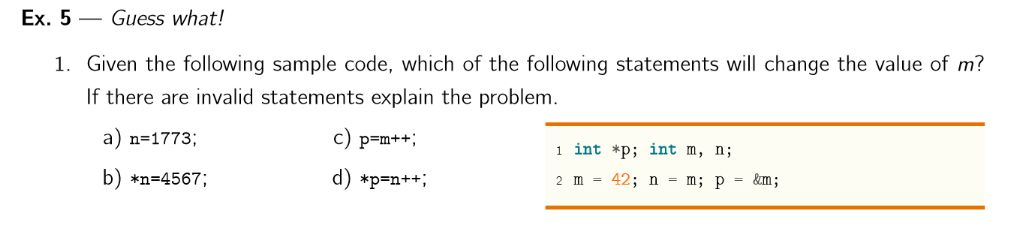
\includegraphics[width=0.75\textwidth]{ex5_0.png}
	\end{figure}
	
\end{frame}

\begin{frame}{Exercise 5}
    \begin{figure}
		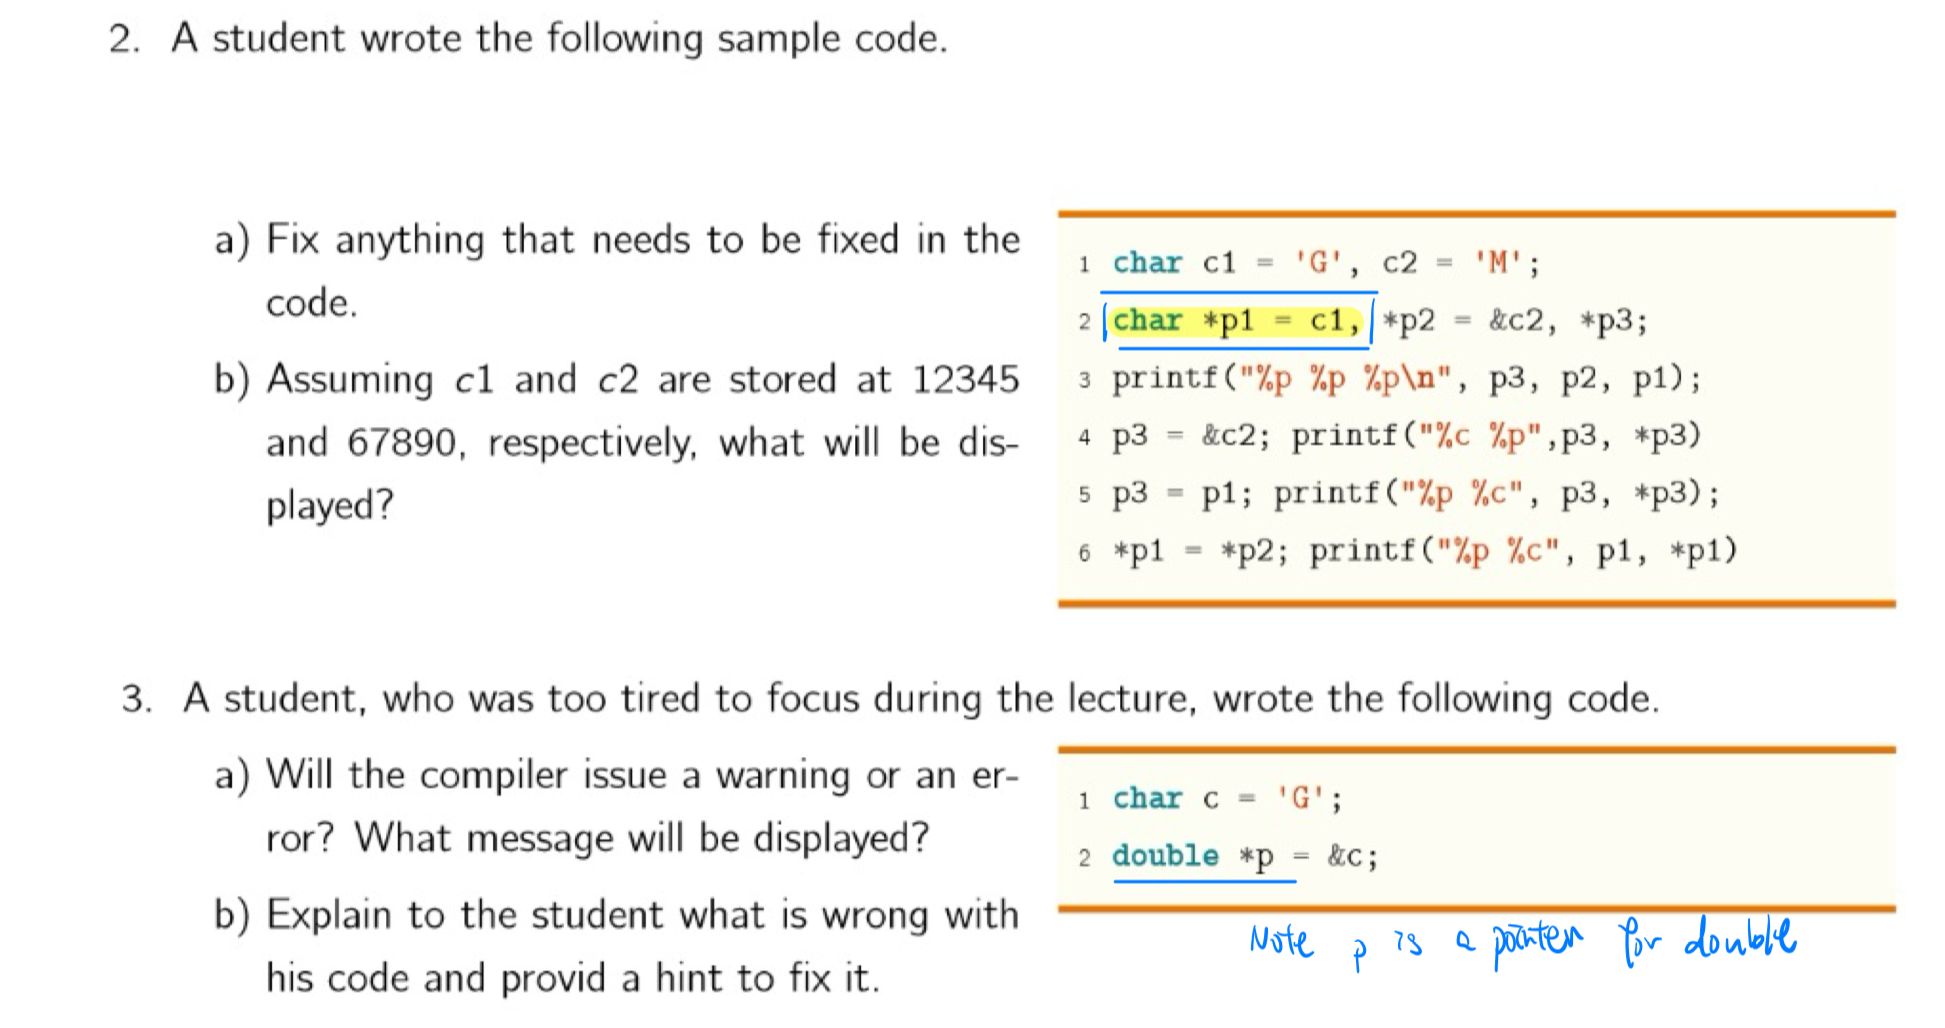
\includegraphics[width=0.75\textwidth]{ex5.png}
	\end{figure}
\end{frame}

\begin{frame}{Exercise 6}
    
\end{frame}

\begin{frame}{Exercise 6}
    \begin{figure}
		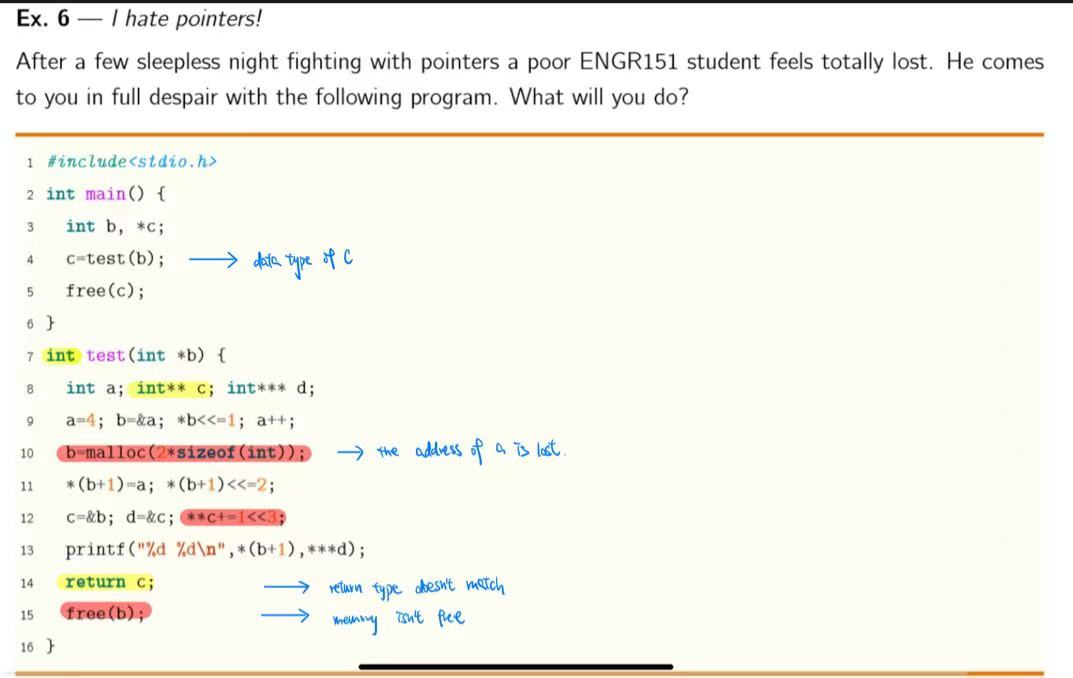
\includegraphics[width=0.75\textwidth]{ex6.jpg}
	\end{figure}
\end{frame}

\section{Referencing}

\begin{frame} % Use [allowframebreaks] to allow automatic splitting across slides if the content is too long
	\frametitle{References}
	
	\begin{itemize}
    \item Manuel. \textit{c5.pdf}. JI Canvas, 2024. \href{https://jicanvas.com/courses/917/files/folder/lectures?preview=333615}{[Link]}.

    \item Manuel. \textit{w5.pdf}. JI Canvas, 2024. \href{https://jicanvas.com/courses/917/files/folder/worksheets?preview=333633}{[Link]}.
\end{itemize}
\end{frame}

%----------------------------------------------------------------------------------------
%	CLOSING SLIDE
%----------------------------------------------------------------------------------------

\begin{frame}[plain] % The optional argument 'plain' hides the headline and footline
	\begin{center}
		{\Huge The End}
		
		\bigskip\bigskip % Vertical whitespace
		
		{\LARGE Questions? Comments?}
	\end{center}
\end{frame}

%----------------------------------------------------------------------------------------

\end{document} 